\chapter{Result}
Now we can use our method to determine $dS/dt$, $Pre$, $ET$ and $R$. After that, we can combine these results and discuss the trend of water storage in Ob basin and the reason for it.
\section{Equivalent water height}
As mentioned in chapter 3, We have GRACE and GRACE-FO data from 4 data centers, which are CSR, GFZ, ITSG and JPL. We can plot the total water storage anomaly from 2002 to 2019. we can see in \ref{fig:4centers} that the trends of 4 curves suit each other well. By using the methods mentioned in \ref{sec:Gaussmarkov} we can generate one timeseries with their uncertainty in this period.
\begin{figure}[htbp]
	\centering
	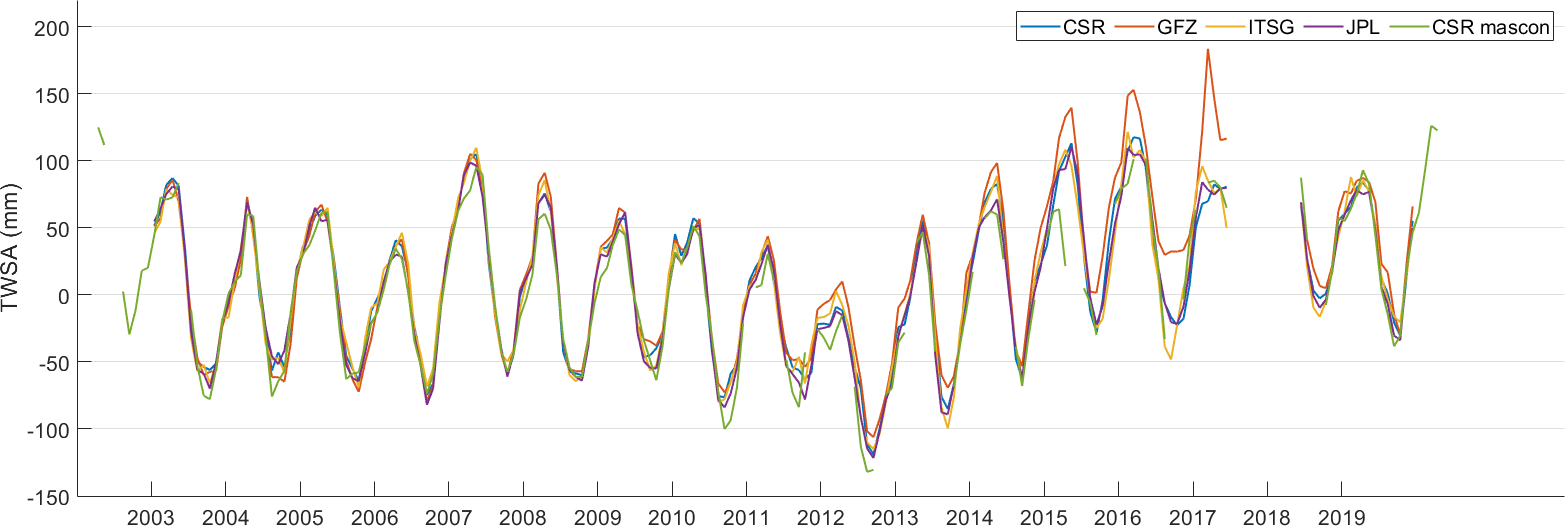
\includegraphics[width=0.9\textwidth]{TWSAall} % Datei in "bilder/" bei LaTeX: eps, bei PDFLaTeX: jpg (o.ä.) 
	\caption{Total water storage anomalie from CSR, GFZ, ITSG and JPL between 2002 and 2020} 
	\label{fig:4centers}
\end{figure}
% figure 4 data centers label(fig:4centers)

Since Ob basin is a quite big area, it is necessary to confirm if the behavior of the total water storage are identical in the whole area, we can divide the whole area in many grids 

% text needs to be finished,  label(fig:grid of ob)

From the timeseries of the TWSA we see an obvious positive trend from 2013 to 2015. Thus, the whole period can divide into 3 phases. In order to find the changing points, we first plot the $dS/dt$ \ref{fig:dsdtall} by using the equation \ref{eq:dsdt}. With the help of the matlab functions \textit{movmean} and \textit{ischange} we can see the mean value of $dS/dt$ between 2013 and 2015 are much bigger than other periods, which confirms our assumption.  

% dsdt figure \label(fig:dsdtall)

\section{Precipitation}
It was mentioned in chapter 3 that we have precipitation data from 9 resources \ref{fig:allpre}, and one timeseries with uncertainty can be generated by combining them. The spatial behavior of precipitation in this area is also interesting to us. \\\\
Since we have already divide the whole period into 3 phases, we are interested what we see the trends of precipitations in this 3 phases.

% all precipitation in one 
\section{Evatranspiration}
Just as precipitation, we present the evatranspiration temparally ans spatially and cut the timeseries in to 3 small periods.

\section{Runoff}
\subsection{Runoff from global datasets}
Like precipitation and evatranspiration, we have many models to present the runoff, we can also show them in a way we did for precipitation and evatranspiration. However, as mentioned in \ref{sec:runoff}, we have in-situ data till 2010, we then can calculate the root-mean-square-error for the models we have. \ref{tab:rmse}.\\\\
Then, by analyzing them using the CDF, we found that most of them are not ideal, so, we need to find a better way to present the runoff.
\subsection{Estimating runoff using quantile function and satellite altimetry}
 As mentioned in \ref{sec:runoff}, we can use the satellite to determine the water level height in Ob basin \ref{fig:waterlevelheight}, and we also have the in-situ data\ref{fig:insitu}, using the methods in, this 